\chapter{Revisión de la literatura}\label{chap:2}

En este capítulo se recopila los hallazgos en la literatura científica sobre los que se apoya este TFG. Se parte de la panorámica general de las redes LPWAN aplicadas a IoT, se profundiza en la capa física de LoRa, el estándar LoRaWAN, se identifican sus usos y limitaciones; se analiza la seguridad en este tipo de redes, se presenta alternativas a LoRaWAN como redes P2P y por último, se examinan las propuestas, como este trabajo, plantean mecanismos de acceso al medio alternativos sobre la capa física LoRa, así como aplicaciones prácticas basadas en LoRa y ESP32.

\section{Redes LPWAN}

Tradicionalmente, la conectividad inalámbrica para sistemas embebidos y redes de sensores se ha desarrollado a través de dos categorías principales de redes, cada una con limitaciones marcadas para escenarios de amplio alcance y bajo consumo.

Por un lado, las redes de área personal y local (WPAN/WLAN), Tecnologías como Bluetooth, Wi-Fi y Zigbee; concebidas para altas tasas de transmisión o entornos locales reducidos cuya distancia de cobertura es un radio entre 10 y 100 metros. Y por otro lado, las redes celulares tradicionales, es decir: 2G, 3G, 4G o 5G. Estas proporcionan una amplia cobertura geográfica y están optimizadas para transportar datos de alta velocidad y voz. Esto conlleva un alto consumo energético y por ende, un coste de operación que no es asumible para nodos alimentados por batería. 

Para superar estas limitaciones surge el paradigma de las redes de área amplia y bajo consumo LPWAN (\textit{Low Power Wide Area Network}). LPWAN se define como una clase de estándares y soluciones inalámbricas diseñadas para transmitir paquetes de datos pequeños (10--1000~bytes) a velocidades reducidas (0,1--250~kbps), priorizando la máxima eficiencia energética y una distancia de transmisión extensa.

LPWAN se fundamenta en los siguientes principios:

\begin{itemize}
    \item Una autonomía energética prolongada. Se espera que los nodos operen durante 10 o más años con baterías comerciales (pilas AA o de botón).
    
    \item Un gran alcance de señal. Los enlaces de comunicación deben ser directos sin línea de visión entre 1 y 5 km en entornos urbanos densos y entre 10 y 40 km en zonas rurales despejadas.

    \item Gran capacidad y escalabilidad. Se debe poder prestar servicio a un número masivo de dispositivos sin degradar la calidad del servicio.

    \item Bajo coste de fabricación y despliegue. La arquitectura Hardware debe estar simplificada para no conllevar un coste superior a 7 USD, aproximadamente.
\end{itemize}

Cuando se habla de LPWAN existen dos divisiones según el espectro radioeléctrico en el que operan. Existen las \textbf{Tecnologías de espectro licenciado}, aquellas desarrolladas bajo los estándares de 3GPP, es decir, operan sobre la infraestructura celular existente. Entre ellas, está narrowband IoT (NB-IoT). NB-IoT se caracteriza por trabajar en bandas LTE licenciadas y requiere de infraestructura móvil comercial, por lo que utilizarla implica asumir unas cuotas de suscripción a operadores de telecomunicaciones. A su vez, existen LTE-M, que ofrece mayor ancho de banda y soporte de movilidad a costa de un consumo energético mayor, y EC-GSM-IoT, que adapta la infraestructura GSM existente a dispositivos IoT.

Por otro lado, están las \textbf{Tecnologías de espectro no licenciado} aprovechan bandas de frecuencia libre de uso industrial, científico y médico (ISM), como 433 y 868~MHz en Europa, 915~MHz en América y diversas bandas en Asia. Entre las principales alternativas destaca Sigfox, que emplea banda ultraestrecha (UNB) y depende de un modelo de servicio específico; DASH7, un protocolo abierto orientado a comunicaciones eficientes por eventos, con soporte para distintas topologías de red y LoRa, basada en modulación CSS (\textit{Chirp Spread Spectrum}).

Para aplicaciones de área local o infraestructuras privadas, el despliegue de redes basadas en bandas no licenciadas presentan ventajas frente a las redes móvil licenciadas. Destaca la independencia de operadores y sus gastos asociados al servicio, lo que da lugar a redes privadas e independientes que otorgan una soberanía absoluta de los datos a nivel local. Además, frente a tecnologías locales como Wi-Fi en 2,4~GHz, operar en bandas sub-GHz ofrece menores pérdidas y mayor capacidad de penetración ante obstáculos o paredes de hormigón.

\section{La tecnología LoRa (\textit{Long Range})}

LoRa es una técnica de modulación, propiedad de Semtech, basada en espectro ensanchado por chirrido o \textit{chirp}, CSS. Esta técnica, empleada en radares y en comunicación militar, usa impulsos de radiofrecuencia, donde la frecuencia varía de forma continua e ininterrumpida a lo largo del tiempo, generando los denominados \textit{chirps}. Puede haber \textit{up-chirps} o \textit{down-chirps}. 

La transmisión de datos mediante este mecanismo de modulación consiste en codificar cada símbolo como un desplazamiento cíclico de la frecuencia inicial del \textit{chirp}, de modo que la señal ocupa todo el ancho de banda del canal, muy superior al que requeriría la tasa de datos transmitida~\cite{devalal2018lora}. Por lo que según el teorema de Shannon-Hartley, el incremento del ancho de banda del canal de transmisión, permite operar en entornos con relación señal-ruido (SNR) muy degradados~\cite{song2017internet}. 
En la figura~\ref{fig:css} se muestra un ejemplo donde se visualiza el cambio de frecuencia respecto al tiempo de una trama LoRa.

Este tipo de modulación ofrece gran robustez frente a \textit{multipath}\footnote{\textit{Multipath} es un fenómeno en el que un receptor recibe una señal que proviene de varios caminos distintos debido a fenómenos físicos que ocurren en el medio como reflexión, refracción y dispersión.} y \textit{fading}\footnote{\textit{Fading} es un fenómeno en el cual una señal varía su amplitud o potencia de señal recibida a lo largo del tiempo en la posición del receptor.}.

\begin{figure}[htbp]
    \centering
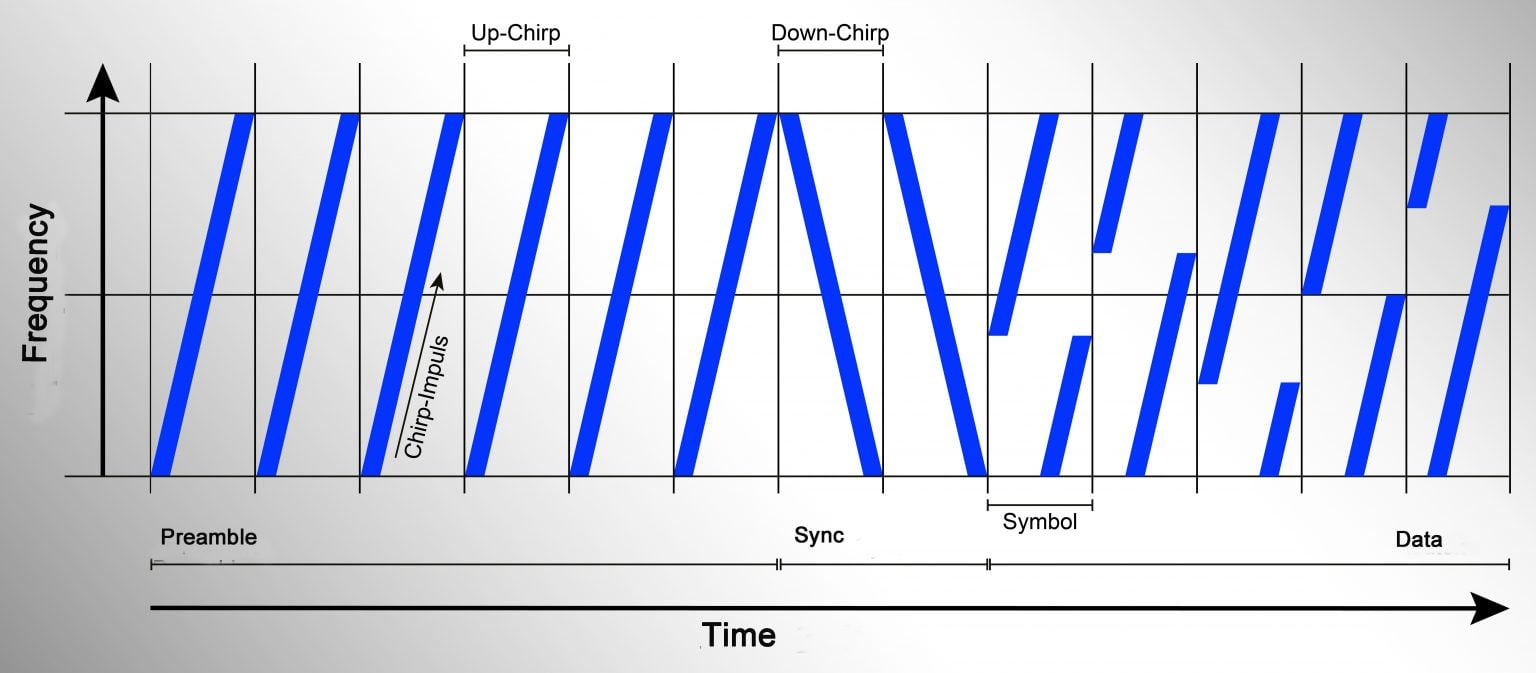
\includegraphics[width=0.7\linewidth]{./imagenes/css.jpg}
    \caption{Gráfico explicativo de modulación CSS~\cite{mokosmart_lora_frequency}. }
    \label{fig:css}
\end{figure}

LoRa se configura mediante la combinación de cuatro parámetros que permiten compensar el compromiso entre alcance, robustez, tasa de transferencia y consumo de energía. Estos son: 

\begin{itemize}
\item \textbf{Factor de dispersión (\textit{Spreading Factor}, SF)}. Puede variar entre SF7 y SF12. Representa el número de bits codificados por cada símbolo. Aumentar el SF duplica la duración de transmisión de un símbolo, mejorando la sensibilidad del receptor y el alcance a cambio de aumentar el Tiempo de permanencia en el aire (\textit{Time-on-Air}, ToA)~\cite{chaudhari2020lpwan}. 

\item \textbf{Ancho de banda (BW)}. Supone el rango de frecuencias asignados al canal. Normalmente se emplea 125~kHz, pudiendo ampliarse hasta 500~kHz. A mayor BW, mayor velocidad de transmisión, pero mayor es la potencia del ruido que se capta en la banda~\cite{devalal2018lora}.

\item \textbf{Tasa de codificación (\textit{Coding Rate}, CR)}. Determina la cantidad de bits de redundancia que se introducen para garantizar la corrección de posibles errores. Puede tomar los valores CR: 4/5, 4/6, 4/7 o 4/8~\cite{arregui2025gatewayfree}.

\item \textbf{Potencia de transmisión ($P_{TX}$)}. Configurable habitualmente entre 2 y 22~dBm según el transceptor, aunque el límite legal lo fija cada sub-banda de la normativa ETSI EN 300 220~\cite{etsien300F2202}. Determina el presupuesto de enlace (\textit{link budget}) del sistema, permitiendo alcanzar un margen de atenuación máximo (\textit{Maximum Allowable Path Loss}, MAPL) superior a los 150~dB~\cite{chaudhari2020lpwan}.
\end{itemize}

En general, la tecnología LoRa opera exclusivamente en la capa física (PHY) del modelo OSI, encargándose de la transmisión y recepción de tramas de radiofrecuencia mediante CSS, pero careciendo de mecanismos nativos para el control de acceso al medio (MAC), direccionamiento de dispositivos o gestión de la topología de red~\cite{arregui2025gatewayfree}. Por este motivo, para constituir una red de comunicaciones completa y funcional se requiere un protocolo de capa superior; en el estándar comercial dominante, esta función la desempeña el protocolo \textit{LoRaWAN}~\cite{devalal2018lora,sornin2015lorawan}.


\section{LoRaWAN y sus limitaciones en entornos locales}

El estándar LoRaWAN (\textit{Long Range Wide Area Network}), mantenido por la LoRa Alliance, define la pila de protocolos de capa superior (Control de Acceso al Medio y capa de red) que opera sobre la capa física LoRa. A diferencia de las redes locales punto a punto o en malla, la arquitectura de LoRaWAN se estructura bajo una topología en estrella de estrellas (\textit{star-of-stars})~\cite{loraalliance_home}. En ella, los nodos finales transmiten mediante enlaces LoRa de un solo salto a una o varios gateways, que reenvían las tramas por una red IP a un servidor de red. Este se encarga de eliminar duplicados, autenticar dispositivos y gestionar parámetros de la red, posteriormente un servidor de aplicación procesa los datos de usuario. En la figura~\ref{fig:lorawanARCH}, se muestra la arquitectura que posee LoRaWAN. 

\begin{figure}[htbp]
    \centering
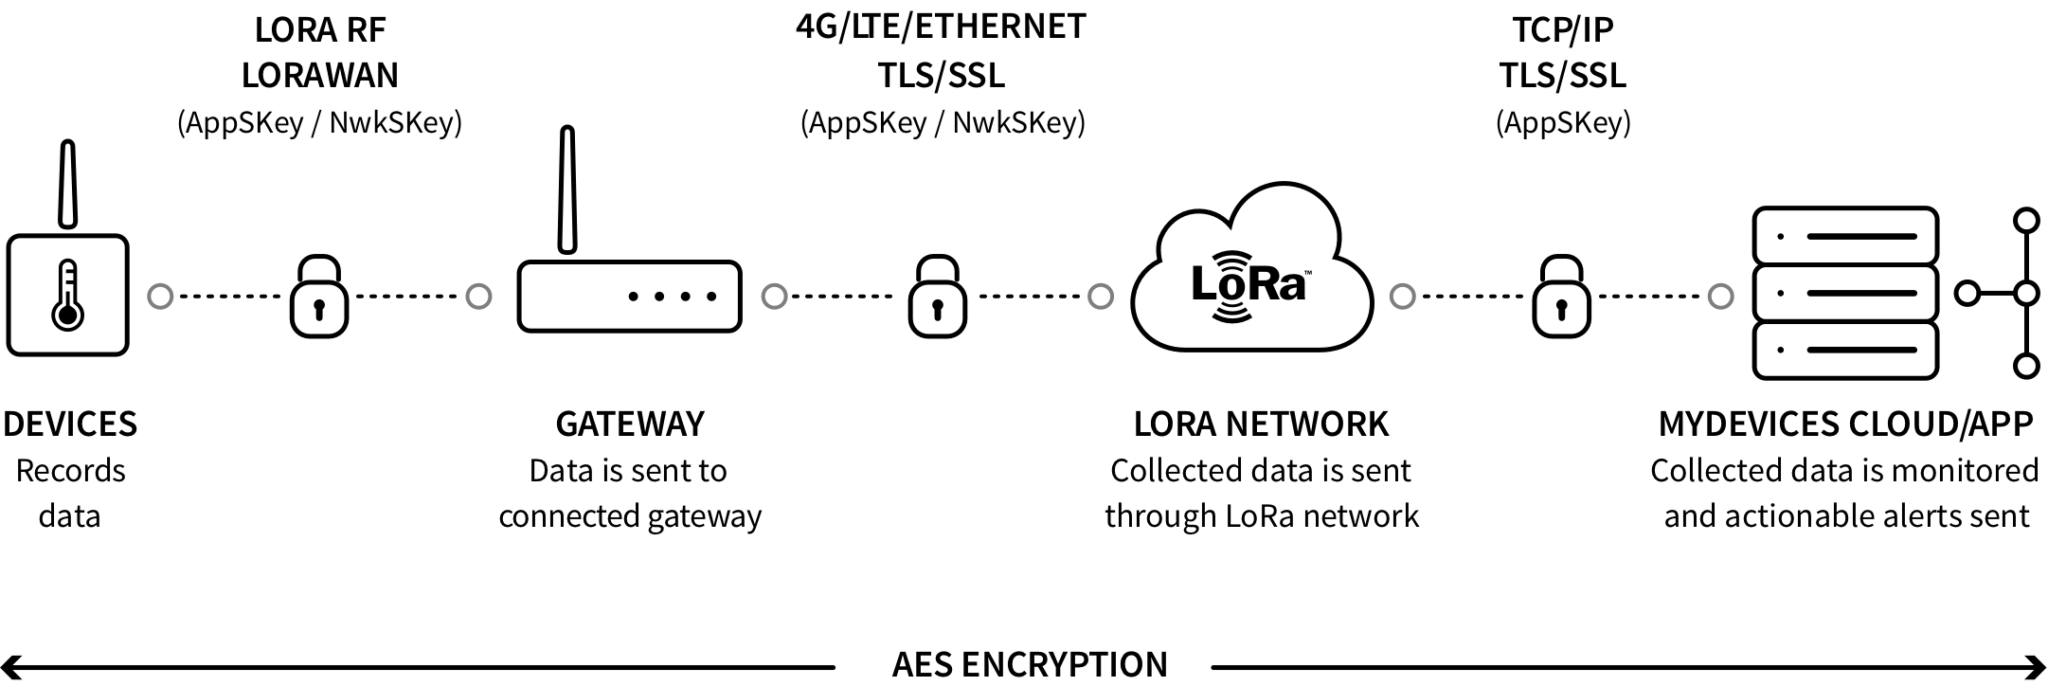
\includegraphics[width=1\linewidth]{./imagenes/lorawan.png}
    \caption{Arquitectura de LoRaWAN y sus distintos componentes~\cite{mydevices_lorawan}. }
    \label{fig:lorawanARCH}
\end{figure}

La especificación define tres clases de dispositivos finales. La clase A, obligatoria
y de menor consumo, abre dos ventanas de recepción tras cada transmisión
ascendente. La clase B añade ventanas de recepción programadas sincronizadas
mediante \textit{beacons}, y la clase C mantiene la recepción abierta de forma
casi continua, a costa de un mayor consumo.
El acceso al medio (MAC) es de tipo ALOHA puro, sin escucha previa del canal, y
queda sujeto a las restricciones de ciclo de trabajo (\textit{duty cycle}) de cada región. Para optimizar la capacidad, el servidor de red puede ajustar dinámicamente el SF y la potencia de los nodos mediante el mecanismo \textit{Adaptive Data Rate} (ADR). Respecto a la seguridad, se emplea AES-128 con dos claves de sesión: una de red, para garantizar la
integridad y autenticidad de los mensajes, y otra de aplicación, que cifra
la carga útil de extremo a extremo~\cite{sornin2015lorawan}.

Estas características convierten a LoRaWAN en una solución consolidada para
despliegues metropolitanos y rurales, pero resulta poco adecuada para una red local con requisitos de baja latencia. Su arquitectura depende de
pasarelas y de un servidor de red, a menudo operados por terceros, lo que añade un
coste de infraestructura~\cite{arregui2025gatewayfree}, y la comunicación descendente queda limitada a las ventanas de recepción de cada clase. Además,
el acceso ALOHA provoca más colisiones al aumentar la densidad de nodos,
lo que degrada la tasa de entrega de paquetes~\cite{adelantado2017limits}, la escalabilidad sigue siendo un reto~\cite{cotrim2020lorawan}.
Estas limitaciones motivan la aparición de alternativas.

\section{Protocolos alternativos y mecanismos de acceso al medio sobre LoRa}

La forma más sencilla de interconexión sobre la capa física LoRa consiste en la comunicación entre pares (\textit{peer-to-peer}, P2P). En este esquema, dos o más microcontroladores intercambian tramas de radiofrecuencia de forma directa sin necesidad de (\textit{gateways}) ni servidores de red en la nube, otorgando al desarrollador un control total sobre el formato de la trama, el control de acceso al medio y la seguridad de la red~\cite{alam2021smart}.

Sin embargo, para gestionar redes locales con múltiples dispositivos surge la necesidad de definir un mecanismo de acceso al medio eficiente. El protocolo estándar LoRaWAN utiliza por defecto un esquema ALOHA no ranurado, en el cual los nodos transmiten de manera asíncrona en el momento en que disponen de datos, sin verificar previamente si el canal radio está ocupado. ALOHA simplifica la arquitectura del nodo final pero sufre una degradación severa por colisiones de paquetes a medida que se incrementa la densidad de la red o la frecuencia del tráfico, impidiendo garantizar el determinismo temporal y la baja latencia que requieren ciertas aplicaciones, como la que se pretende desarrollar en este trabajo.

Para mitigar las limitaciones de ALOHA y evitar colisiones destructivas en el canal inalámbrico, la literatura académica ha explorado, entre otras, dos alternativas en la capa MAC:

\begin{enumerate}
    \item \textbf{Mecanismos basados en división temporal (TDMA / \textit{Slotted MAC})}: Dividen el tiempo de transmisión en ranuras discretas (\textit{time slots}) asignadas individualmente a cada nodo para erradicar las colisiones internas. Entre las propuestas pioneras destaca \textit{LoRaBlink}, basada en un protocolo de recolección en árbol con ranuras temporales~\cite{bor2016lora}, así como arquitecturas coordinadas que implementan sincronización en banda~\cite{farahani2026sdlora} para cumplir con plazos de entrega estrictos (\textit{deadlines}).
    \item \textbf{Mecanismos basados en escucha previa del canal (LBT / \textit{CSMA})}: Evalúan la presencia de portadora (\textit{Listen-Before-Talk}) antes de emitir y aplican temporizadores de espera aleatorios (\textit{backoff}) si el canal está ocupado. Proyectos de código abierto orientados a la mensajería sin infraestructura como \textit{Meshtastic}~\cite{meshtastic} utilizan este enfoque para coordinar nodos distribuidos de forma descentralizada.
\end{enumerate}

A partir de estos principios de acceso y coordinación se han desarrollado tanto mallas P2P sin pasarelas~\cite{berto2021lora} como soluciones multisalto sobre LoRaWAN~\cite{cotrim2020lorawan} y redes en malla (\textit{mesh}) multisalto generales~\cite{pueyo2021beyond}, en las que los nodos retransmiten paquetes de sus vecinos para extender la cobertura evitando la centralización en \textit{gateways}.

En este ámbito, Arregui Almeida \textit{et al.}~\cite{arregui2025gatewayfree} diseñan y validan una red en malla sin \textit{gateway} sobre microcontroladores de consumo ESP32-S3 con transceptores SX1262. Su propuesta integra encaminamiento por vecinos, confirmaciones salto a salto y acceso al canal de tipo \textit{Listen-Before-Talk} (LBT), obteniendo tasas de entrega de paquetes (PDR, \textit{Packet Delivery Ratio}) de hasta el 95\,\% en entornos controlados. Aunque la topología difiere de la arquitectura de área local en estrella prevista para el protocolo a desarrollar, este trabajo valida dos aspectos cruciales: la viabilidad técnica de implementar un protocolo sobre la capa física de LoRa personalizado sobre hardware de bajo coste (ESP32) y la eficacia de la escucha previa LBT como mecanismo de acceso al medio para reducir colisiones.

\section{Seguridad en redes LPWAN}

La seguridad en las redes LPWAN se basa en garantizar confidencialidad, integridad y autenticación de mensajes~\cite{iqbal2018aes}. La especificación de LoRaWAN, basa la seguridad en con doble capa basada en AES-128. La clave de sesión de red (NwkSKey) genera un código de integridad (MIC) de 32 bits sobre la trama, y la clave de sesión de aplicación (AppSKey) cifra la carga útil de extremo a extremo~\cite{sornin2015lorawan}.

Este método posee limitaciones prácticas. En muchos nodos comerciales el microcontrolador se comunica con el transceptor por UART o SPI sin cifrar. Un atacante con acceso al dispositivo puede capturar las claves de sesión y clonar el nodo. Además, el propio canal radio es abierto. Eso lo expone a interferencias deliberadas (\textit{jamming}), el cual es un problema muy presente en IoT~\cite{sigfox2017overview}. Por último, se pueden dar ataques de repetición cuando no se validan los contadores de trama~\cite{vodafone_nbiot}. Ambos ataques permiten, a su vez, ataques tipo \textit{wormhole}, en los que se suprimen mensajes legítimos y se reinyectan paquetes capturados anteriormente~\cite{chacko2018security}.


Tras revisar la literatura científica, se confirma la viabilidad de aplicar mecanismos de seguridad en dispositivos de bajo coste, Iqbal e Iqbal~\cite{iqbal2018aes} exponen un sistema de comunicación punto a punto seguro para microrredes usando AES sobre ESP32 con módulo LoRa, logrando autenticación mediante códigos de autenticación únicos por mensaje con enlaces de larga distancia y bajo consumo. Este resultado es directamente extrapolable a este trabajo, donde se emplea la misma combinación, ESP32 y transceptor LoRa.

\section{Microcontroladores para IoT: el ESP32}

El ESP32, desarrollado por Espressif Systems, se ha consolidado como plataforma de referencia para nodos IoT de bajo coste. Integra un procesador de doble núcleo Xtensa de hasta 240~MHz, memoria SRAM del orden de cientos de KB, buses SPI, UART e I$^2$C, aceleración criptográfica por hardware (AES, SHA y RSA) y conectividad Wi-Fi y Bluetooth~\cite{espressif_esp32_datasheet}. Esta capacidad de cómputo, muy superior a la de microcontroladores de 8 bits como el ATmega328, presentes en Arduino, permite ejecutar sobre el propio nodo una pila de red completa, incluyendo enrutamiento, gestión de tablas de vecinos y cifrado, sin depender de servidores externos.

En aplicaciones prácticas el ESP32 se combina con transceptores sub-GHz de Semtech como el SX1276 o el SX1262 comunicados a través de SPI~\cite{semtech_sx1262_datasheet}. Existen placas comerciales que integran ambos chips, la antena y una pantalla OLED, como las TTGO LoRa32 o la Heltec Wireless Stick V3. Esta última combina un ESP32-S3 con un SX1262 y es la plataforma utilizada por Arregui Almeida \textit{et al.}~\cite{arregui2025gatewayfree} para validar una red \textit{mesh} LoRa sin pasarelas.

\section{Síntesis del capítulo}

En conclusión, la revisión de la literatura muestra que la capa física LoRa permite desarrollar soluciones de comunicación de largo alcance y bajo coste. Aunque LoRaWAN proporciona una solución estandarizada y ampliamente utilizada, sus mecanismos de coordinación y su arquitectura no necesariamente se ajustan a las necesidades de todas las aplicaciones de IoT.


Por otra parte, los trabajos sobre redes P2P, arquitecturas en malla y mecanismos
alternativos de acceso al medio demuestran que es viable implementar protocolos
propios sobre LoRa con hardware de bajo coste como el ESP32. Ninguno de ellos,
sin embargo, reúne a la vez una infraestructura mínima y propia, un acceso al
medio coordinado y una respuesta inmediata en ambos sentidos. A partir de estos
antecedentes, este TFG propone LoRaLAN: un protocolo en estrella de un solo salto,
con una única pasarela gestionada por la propia institución, que no depende de
infraestructura de terceros e integra la seguridad en su diseño.

El objetivo es dar soporte a aplicaciones como la monitorización de aulas y el
registro presencial de la actividad docente en el Centro Universitario de Mérida.
Su viabilidad se evalúa experimentalmente en el Capítulo~\ref{chap:6},
en términos de tasa de entrega de paquetes, latencia y comportamiento ante
transmisiones concurrentes.
